%\section{Wprowadzenie}
\section{Introduction}

%Integracja technologii baz danych z nowoczesnymi metodami
%indukcyjnego generowania wiedzy jest naturalnym kierunkiem rozwoju
%system�w bazodanowych. 

The integration of the database technology with modern inductive methods of
knowledge generation is a natural direction of database systems development.


%Systemy nazywane czasem indukcyjnymi bazami
%danych potrafi� odpowiedzie� nie tylko na pytania, dla kt�rych
%odpowied� znajduje si� w bazie danych, ale r�wnie� na pytania,
%kt�re wymagaj� zsyntetyzowania i zastosowania wiedzy,
%wygenerowanej przez indukcyjne wnioskowanie z fakt�w z bazy danych
%i wcze�niejszej wiedzy~\cite{bib3}. 

Systems which are also referred to as inductive data bases allow finding
answers to questions, to which the replies are in the database,
and also to questions which demand synthesis and knowledge generated
by inductive deduction from facts from database and formerly gained knowledge.

% Schemat typowej indukcyjnej
% bazy danych przedstawiony jest na rysunku~\ref{fig:inddb}.
A schema of a typical inductive database was presented on the picture
~\ref{fig:inddb}.

\begin{figure}[!ht]
    \centering
        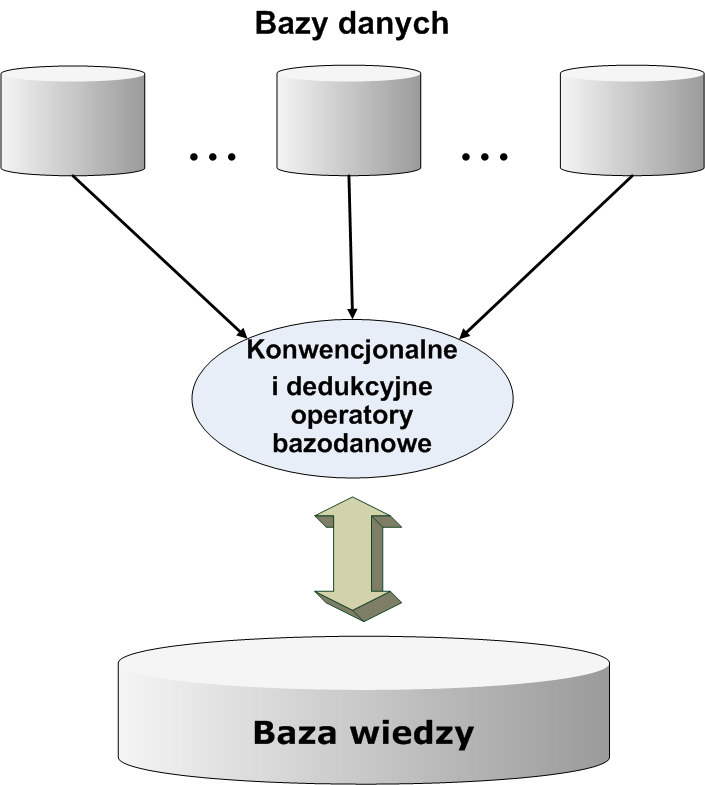
\includegraphics[width=\linewidth]{img/knowledge_mining.png}
%    \caption{Indukcyjna baza danych~\cite{bib2}}
    \caption{Inductive data base~\cite{bib2}}
    \label{fig:inddb}
\end{figure}



%W pierwszej cz�ci pracy przedstawione zosta�y wybrane istniej�ce
%�rodowiska wspieraj�ce uruchamianie algorytm�w uczenia maszynowego.
Selected environments, which allow running the algorithms of machine learning,
were described in the first part of the article.

%Dalej opisano za�o�enia, a~nast�pnie architektur� i wybrane aspekty
%implementacji komponentowej realizacji indukcyjnej bazy danych --
%platformy \emph{Salomon}.

Firstly the assumptions, then the architecture and various implementation
aspects of component realization of the inductive database -- the \emph{Salomon}
platform are described in the following part of the article.

%  Dzi�ki budowie modu�owej uda�o si� uzyska�
%du�o wi�ksz� elastyczno�� systemu w stosunku do opisanych wcze�niej
%rozwi�za�.

The last part of the article shows the possibilities of using the platform
for teaching the decision trees.
%  Ostatnia cz�� pracy prezentuje mo�liwo�ci wykorzystania
%platformy do uczenia drzew decyzyjnych.

Thanks to the modular structure much better system flexibility
, in comparison to the systems described below, was achieved.

